\chapter{Applications and Examples}
\label{cha:applic}
The final major chapter of this work will first compare the TRK statistic/suite to similar methods in \S\ref{sec:compare}, and schematically demonstrate the improvements over thereof of TRK. From here, I will demonstrate the TRK fitting algorithms in practice within \S\ref{sec:extincfits}, by performing TRK fits with models that involve parameters related to the dust-extinction of interstellar light.
\section{Comparison to Similar Algorithms}
\label{sec:compare}
Surprisingly, there are not very many algorithms that can be used to fit models to data that has uncertainty in two dimensions (even fewer that can account for both intrinsic and extrinsic uncertainties). To further examine the usefulness of the TRK suite, I will begin by comparing it to various similar algorithms, and showing how, overall, it is usually the most robust and general choice. First, I will discuss a non-Bayesian least-squares algorithm, then we will explore two Bayesian algorithms that are similar, but inferior to TRK.

Perhaps the most well known/most-used 2D-uncertainty fitting method is Orthogonal Distance Regression/ODR, also known as Total Least Squares\footnote{For example, one of the most commonly used implementations of ODR is the \texttt{scipy.odr} Python module (see \url{https://docs.scipy.org/doc/scipy/reference/odr.html}.)}. ODR is a nonlinear least-squares regression method that minimizes the distances between the datapoints and the fitted curve along some direction(s) determined by the error bars of the data, e.g. \textcite{brown1990odr}. Despite being heavily used, there are a number of downsides to this method as compared to the TRK statistic, for example:
\begin{enumerate}
    \item There is no obvious method to include/parameterize extrinsic scatter/slop in the dataset with ODR.
    \item There is no general method to incorporate ODR into a Bayesian formalism, e.g. including priors, that we have found.
    \item As shown by \textcite{odrscale}, ODR is \textit{not} scalable/scale invariant, i.e. changing the units of the axis/axes will result in different, unequivalent fits.
\end{enumerate}
As such, when a rigorous, flexible and generalizable fitting algorithm is desired over pure computational speed, TRK will be a better choice over ODR.

% ODR is actually invertible, I checked

As described in \S\ref{sec:likelihood}, the choice of the arbitrary rotated coordinates $(u_n,v_n)$ and therefore the factor $\dv{u_n}{x}$ in Equation \eqref{eq:likegen}---the likelihood function in our general case---will be what defines a given statistic's criteria for a best fit. \textcite{trotter} showed that various choices of $\dv{u_n}{x}$ will lead to different statistics with varying properties. There exist two other 2D-uncertainty Bayesian model-fitting statistics in the literature, both of which are thoroughly explored and compared to the TRK statistic in Trotter's work: that of \textcite{d05fits}, or D05, and that of \textcite{r01}, or R01. In the following, we will summarize Trotter's work of showing how both of these statistics are derived from certain choices of $\dv{u_n}{x}$, and comparing them to the TRK statistic.

The D05 statistic of \textcite{d05fits} is defined by setting $\diff u_n = \diff x$, i.e. $\dv{u_n}{x}=1$ in Equation \eqref{eq:likegen}, giving a likelihood function of
\begin{align}\label{eq:D05}
\mathcal{L}^\mathrm{D05} & \propto \prod_{n=1}^{N}{ \frac{1}{\sqrt{m_{t,n}^2\Sigma_{x,n}^2+\Sigma_{y,n}^2}}\exp\left\{-\frac{1}{2}\frac{\left[y_n-y_{t,n}-m_{t,n}(x_n-x_{t,n})\right]^2}{m_{t,n}^2\Sigma_{x,n}^2+\Sigma_{y,n}^2}\right\}} \nonumber \\
-2\ln\mathcal{L}^\mathrm{D05} & =  \sum_{n=1}^{N}{\frac{\left[y_n-y_{t,n}-m_{t,n}(x_n-x_{t,n})\right]^2}{m_{t,n}^2\Sigma_{x,n}^2+\Sigma_{y,n}^2}} + \sum_{n=1}^{N}\ln(m_{t,n}^2\Sigma_{x,n}^2+\Sigma_{y,n}^2) + C \, .
\end{align}
From \textcite{trotter}, ``The D05 statistic can be seen to be analogous to a one-dimensional $\chi^2$ statistic in $y$, where the difference between the model and the datapoint is the difference between the tangent line at $x=x_n$ and $y_n$, and where the $1\sigma$ uncertainty in the convolved datapoint is replaced by the quadrature sum of $\Sigma_{y,n}$ and $\Sigma_{x,n}$ projected into the $y$-direction using the slope $m_{t,n}$. D05 differs from a traditional $\chi^2$ statistic in that the denominator of the argument of the exponential, and the prefactor of the exponential are themselves functions of the slops $(\sigma_x,\sigma_y)$, which are treated as free model parameters.'' However, as shown by Trotter, while D05 is scalable and reduces to a 1D $\chi^2$-like statistic in the limit of $\Sigma_{x,n}\rightarrow 0$, it is \textit{not} invertible, unlike the TRK statistic.

The R01 statistic of \textcite{r01} is defined using $\diff u_n = \diff s_n$, where $\diff s_n\equiv\sqrt{\diff x^2+\diff y^2}$ is parallel to the tangent line with slope $m_{t,n}$, giving $\dv{u_n}{x}=\sqrt{1+m_{t,n}^2}$. Using Equation \eqref{eq:likegen}, this results in a likelihood of
\begin{eqnarray}\label{eq:R01}
\mathcal{L}^{\mathrm {R01}} & \propto & \prod_{n=1}^{N}{\sqrt{\frac{1+m_{t,n}^2}{m_{t,n}^2\Sigma_{x,n}^2+\Sigma_{y,n}^2}}\exp{\left\{-\frac{1}{2}\frac{\left[y_n-y_{t,n}-m_{t,n}(x_n-x_{t,n})\right]^2}{m_{t,n}^2\Sigma_{x,n}^2+\Sigma_{y,n}^2}\right\}}} \nonumber \\
-2\ln\mathcal{L}^{\mathrm{R01}} & = & \sum_{n=1}^{N}{\frac{\left[y_n-y_{t,n}-m_{t,n}(x_n-x_{t,n})\right]^2}{m_{t,n}^2\Sigma_{x,n}^2+\Sigma_{y,n}^2}} \nonumber \\
& & - \sum_{n=1}^{N}{\ln\left(\frac{1+m_{t,n}^2}{m_{t,n}^2\Sigma_{x,n}^2+\Sigma_{y,n}^2}\right)} + C \, .
\end{eqnarray}
The R01 statistic was designed to be invertible (\textcite{r01}); however, as shown in \textcite{trotter}, although it \textit{is} invertible, the statistic is neither scalable, nor reduces to a 1D $\chi^2$-like statistic in the limit of $\Sigma_{x,n}\rightarrow 0$.


While D05 is scalable and reduces to a 1D $\chi^2$-like statistic in the limit of $\Sigma_{x,n}\rightarrow 0$, it is not invertible. Similarly, while R01 is invertible, it is not scalable and it does not reduce to a 1D $\chi^2$-like statistic in the aforementioned limit. The TRK statistic, however, manages to be the best of both worlds, as it is invertible (see \S\ref{sec:invertibility}), reduces to a 1D $\chi^2$-like statistic (see \S\ref{sec:tgtpts} and \textcite{trotter}), and by using the scale optimization algorithm of \S\ref{sec:scaleop}, can be made to be scale invariant.

\section{Interstellar Extinction Model Parameter Fits}
\label{sec:extincfits}
In \textcite{trotter}, various TRK fits were made to model correlations between parameters that describe empirical fits to the observed spectral extinction by dust of light originating from stars in the Milky Way and Magellanic Clouds. These fits served to be a ``proof of concept'' of Trotter's ``science code'' implementation of the TRK statistic. Now that I have developed the TRK statistic in the form of a much more automated, generalizable and computationally efficient implementation, I will redo these fits, with updated datasets, as follows.

The aforementioned dust extinction models were first formalized in \textcite{cardelli1989relationship} (CCM) and \textcite{fitzpatrick1988analysis} (FM), and are summarized and described in Figure \ref{fig:ccmfm}. In the following section, I will explore the relationships between the empirical parameters $c_1$, $c_2$, $c_3$, and $\gamma$ of the CCM/FM model. 
\begin{figure}
    \centering
    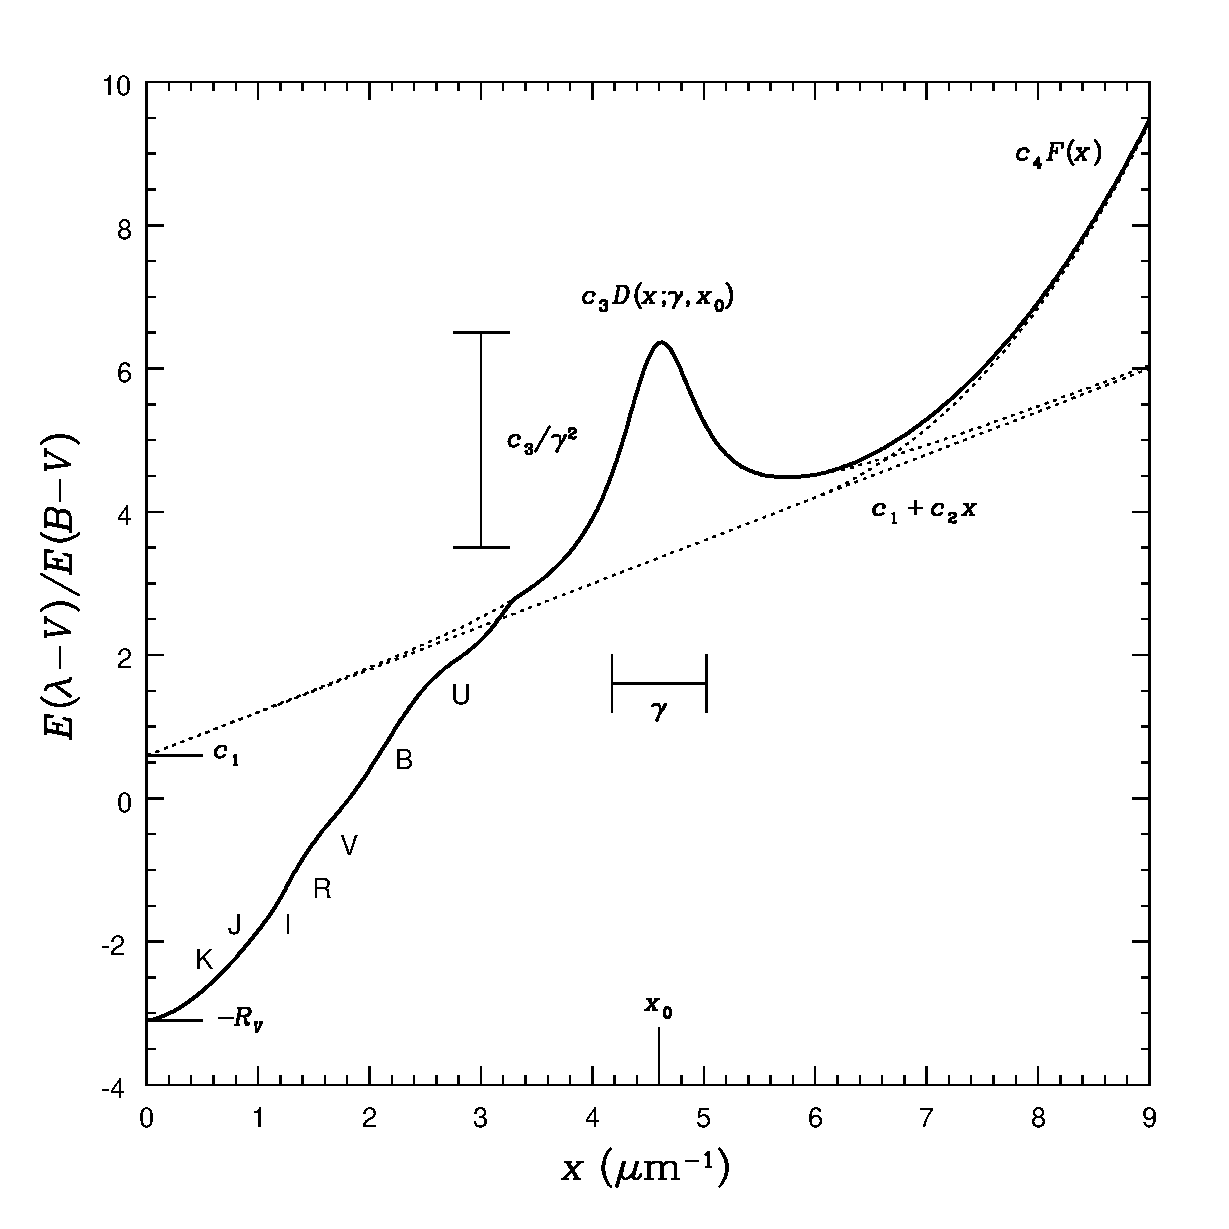
\includegraphics[width=1.0\linewidth]{figures/ccmfm.eps}
    \caption{From \textcite{trotter}, the combined CCM and FM extinction model curve along a typical Milky Way line of sight. The $y$-axis is defined to be the ratio between the $\lambda-V$ color excess $E(\lambda-V)$ at a given wavelength $\lambda$, and the $B-V$ color excess $E(B-V)$, where the color excess is defined as the difference, in magnitudes, of the absorption due to dust at two given wavelengths. In this case, $B$ and $V$ correspond to wavelengths in the middle of standard blue and visible photometric filters. The color excess ratio plotted on the $y$-axis is thus proportional (with an offset) to the magnitude of dust extinction at a given wavelength $\lambda$. The $x$-axis is proportional to the inverse of $\lambda$, specifically $x\equiv(\lambda/1 \text{ $\mu$m})^{-1}$, or, equivalently, proportional to frequency. As shown, the parameters $c_1$ and $c_2$ describe the intercept and slope of a linear component of the model. The parameter $\gamma$ parameterizes the width of the ``bump'' in the center of the model (also known as the ``UV bump''), while the parameter $\text{BH}\equiv c_3/\gamma^2$ describes the height of this bump.}
    \label{fig:ccmfm}
\end{figure}
As described in \textcite{trotter}, there are known correlations between $c_1$ and $c_2$, and between the so-called ``bump height'' parameter $\text{BH}\equiv c_3/\gamma^2$ (see Fig \ref{fig:ccmfm})  and $c_2$. The dataset that was fit to in \textcite{trotter} is comprised of extinction parameter measurements from 417 stars in the Milky Way, from \textcite{valencic04}, and 23 stars from the Large and Small Magellanic Clouds, from \textcite{gordon03}. This dataset contains values and symmetric error bars for $c_1, c_2, c_3$ and $\gamma$ (as well as other CCM/FM parameters that don't concern our fits), through which Trotter derived values and error bars for $\text{BH}$ through standard propagation of uncertainty\footnote{The parameters from \textcite{valencic04} were calculated with a normalization given the parameter $R_V$ by \textcite{trotter}, and their error bars were assigned through standard propagation of uncertainty.}. 

For this thesis, following a thorough search through the literature, I updated the full dataset with data from 328 stars in the Milky Way from \textcite{newdatafitzpatrick2007analysis}, and one star in M31 from \textcite{m31dataclayton2015new}. %\footnote{Note that a few of these datapoints have no errorbars supplied in one or more directions; in this case, I exclude such datapoints from fitting, as if slop parameters are zero or close to zero, the prefactor of the TRK likelihood (Equation \eqref{eq:TRK}) can ``blow-up'', leading to a numerically infinite likelihood.}. 
From here, I redid the fits of the models describing $c_1$ vs. $c_2$ and $\text{BH}$ vs. $c_2$ that were formulated and presented in \textcite{trotter}, with the updated dataset of $N=729$ values of $\{c_1, c_2, \text{BH}\}$ with symmetric error bars (again computing error bars for $\text{BH}\equiv c_3/\gamma^2$ with standard propagation of uncertainty). Following \textcite{trotter}, I assigned some weight $w_n$ to each $n^\text{th}$ datapoint that is inversely proportional to the integral of the sum of all $N$ of the intrinsic Gaussian $c_2$ distributions of the datapoints, weighted by the Gaussian of the corresponding $c_{2,n}$, i.e.
\begin{equation}\label{eq:c2weight}
w_n\propto\left[\int_{-\infty}^\infty\left(\mathcal{N}(c_2|c_{2,n},\sigma_{c_2,n})\sum\limits_{i=1}^N\mathcal{N}(c_2|c_{2,i},\sigma_{c_2,i})\right)\diff c_2\right]^{-1},
\end{equation}
and then normalizing the weights such that the minimum weight is unity\footnote{\label{footnote:weighting}Datapoint weights $\{w_n\}$ are implemented into the TRK likelihood by multiplying the terms within the summations of the lower line of Equation \eqref{eq:TRK} by $w_n$, which translates to a \textit{weighted} likelihood of 
$\displaystyle\mathcal{L}^{\mathrm {TRK}} \propto \prod_{n=1}^{N}{ \left(\frac{m_{t,n}^2\Sigma_{x,n}^2+\Sigma_{y,n}^2}{m_{t,n}^2\Sigma_{x,n}^4+\Sigma_{y,n}^4}\right)^{\displaystyle w_n/2}\times\exp\left\{{-\frac{1}{2}w_n\frac{\left[y_n-y_{t,n}-m_{t,n}(x_n-x_{t,n})\right]^2}{m_{t,n}^2\Sigma_{x,n}^2+\Sigma_{y,n}^2}}\right\}}$.}. This weighting is used in order to increase the weight of/``oversample'' the occasional high $c_2$ datapoint (\textcite{trotter}). From here, I ran TRK fits for $c_1$ vs. $c_2$ and $\text{BH}$ vs. $c_2$, that will be described and presented in the following subsections.

\subsection{Fitting $c_1$ vs. $c_2$}
From \textcite{trotter}, the parameters $c_1$ and $c_2$ are strongly linearly correlated, as the two describe the intercept and slope of a linear component of the FM extinction model. The model distribution that I will use to parameterize this correlation, defined by Trotter, has a model curve $y_c(x;\vartheta_m)$ of the form
\begin{equation}\label{eq:c1c2model}
    c_{1,c}(c_2;\vartheta_m)=b^{c_1}+m^{c_1}\left(c_2 - c_2^{p_{c_1}}\right),
\end{equation}
where $\vartheta_m=\{b^{c_1}, m^{c_1}\}$ are the model parameters and $c_2^{p_{c_1}}$ is the pivot point of the model, of which the choice of affects the amount of correlation between $b^{c_1}$ and $m^{c_1}$ (see \S\ref{sec:pivot}).

To fit this model to the dataset, I first ran the scale optimization algorithm of \S\ref{sec:scaleop} to determine the optimum fitting scale $s_0$. Next, I ran the parameter correlation removal/pivot point-finding algorithm of \S\ref{sec:pivot} to determine the pivot point $c_2^{p_{c_1}}$ that minimizes the correlation between $b^{c_1}$ and $m^{c_1}$. From here, I determined the best fit model and $(x-,y-)$slop parameters $\vartheta_m=\{b^{c_1}, m^{c_1}\}$ and $\{\sigma_{c_2}^{c_1}, \sigma_{c_1}\}$, respectively using the Downhill Simplex method of \S\ref{sec:simplex} at $s_0$\footnote{Note that I was able to run the scale optimization before finding the pivot point because fitting scales are invariant of choice of pivot point, as they don't affect the extreme scale limiting behavior of slops, e.g. \textcite{trotter}.}. Finally, I used the Adaptive MCMC and Bar-Lowering methods of \S\ref{sec:MCMC} to sample the distribution of the model and slop parameters, and compute their uncertainties, respectively. 

The numerical results of this fit are given in Table \ref{table:c1c2}, while the fit is plotted in Figure \ref{fig:c1c2_data} with generated model and slop parameter distributions shown in Figure \ref{fig:c1c2_params}. In Figure \ref{fig:c1c2_data}, note the strong correlation between $c_1$ and $c_2$, as expected. Also, note that because the pivot point-finding routine was used to minimize the correlation between $b^{c_1}$ and $m^{c_1}$, the confidence ellipse for these two parameters (top, center of Figure \ref{fig:c1c2_params}) is not tilted, indicating the removal of correlation between them. Finally, also note in this figure that the two slop parameters $(\sigma_{c_2}^{c_1}$ and $\sigma_{c_1})$ are also uncorrelated, again evidenced by a non-tilted confidence ellipse (bottom, center).

\begin{figure}
    \centering
    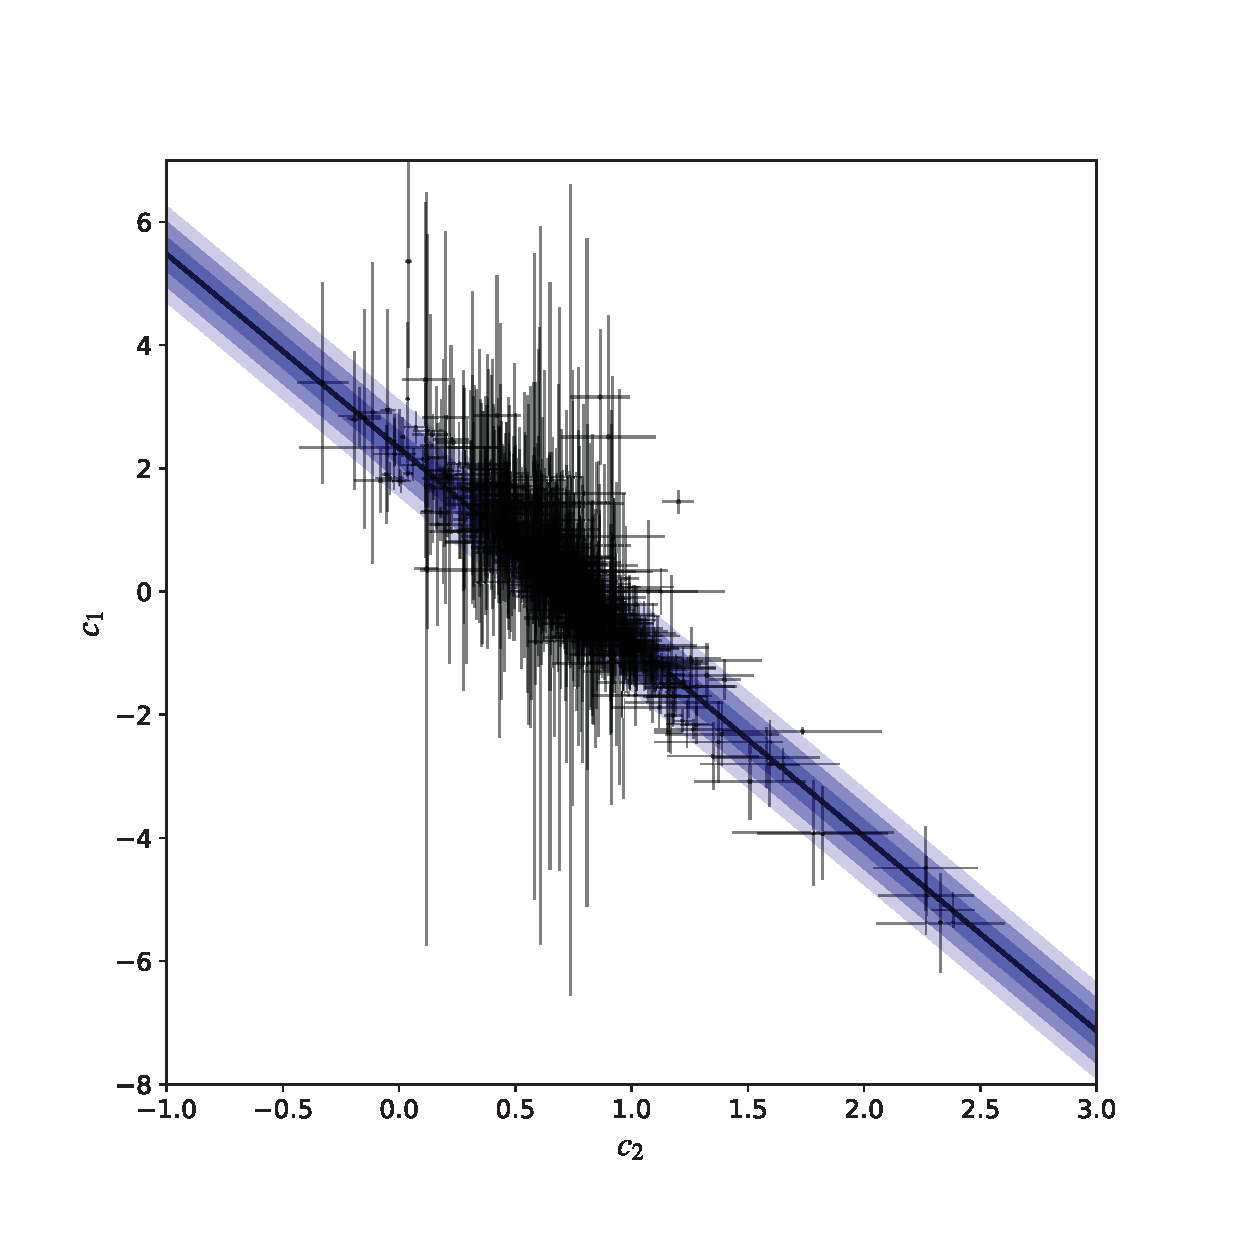
\includegraphics[width=1.0\linewidth]{figures/c1c2_data.eps}
    \caption{Observed $c_1$ vs $c_2$ data from \textcite{valencic04}, \textcite{gordon03}, \textcite{newdatafitzpatrick2007analysis}, and \textcite{m31dataclayton2015new}, plotted with linear TRK fit modeled by Equation \eqref{eq:c1c2model}. Shaded regions indicate the $1-$, $2-$ and $3\sigma$ slop confidence regions of the model distribution, given best fit slop values of Table \ref{table:c1c2} and plotted according to footnote \ref{footnote:modelcurvebands} on page \pageref{footnote:modelcurvebands}.}
    \label{fig:c1c2_data}
\end{figure}

\begin{figure}
    \centering
    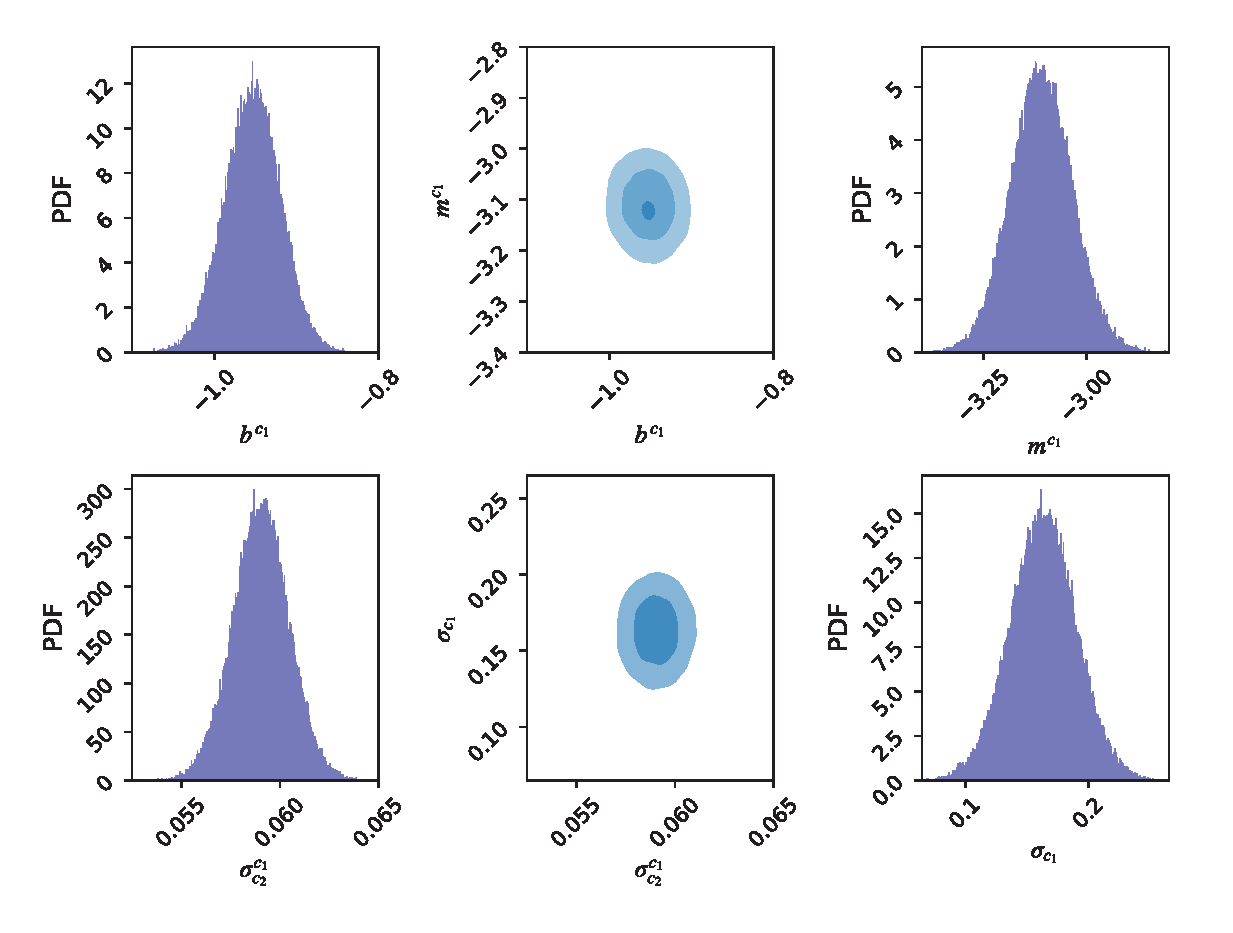
\includegraphics[width=1.0\linewidth]{figures/c1c2_params.eps}
    \caption{MCMC-generated (\S\ref{sec:MCMC}) probability distributions for $c_1$ vs. $c_2$ (Equation \eqref{eq:c1c2model}) model (top) and slop/extrinsic scatter (bottom) parameters. Parameter confidence ellipses (center) with $1-$, $2-$ and $3\sigma$ regions show joint posterior probabilities with respect to the parameters plotted on either side. The pivot-point finding algorithm of  \S\ref{sec:pivot} was used to remove correlation between model parameters.}
    \label{fig:c1c2_params}
\end{figure}

\begin{table}
\label{table:c1c2}
\caption{Best-Fit Asymmetric Gaussian Parameter Values For $c_1$ vs. $c_2$ Model (Equation \eqref{eq:c1c2model})}
\centering
\vspace{0.3cm}
\begin{tabular}{@{}lcccc@{}}
\toprule
Parameter Type   & Parameter            & Value    & \begin{tabular}[c]{@{}c@{}}$+1\sigma$\\ Width\end{tabular} & \begin{tabular}[c]{@{}c@{}}$-1\sigma$\\ Width\end{tabular} \\ \midrule
Model Parameters & $b^{c_1}$            & $-0.9052$  & 0.0350                                                     & $-0.0376$                                                    \\
                 & $m^{c_1}$            & $-3.1519$  & 0.0778                                                     & $-0.0762$                                                    \\
Pivot Point      & $c_2^{p_{c_2}}$      & 1.0247 & $\ldots$                                                   & $\ldots$                                                   \\
Slop Parameters  & $\sigma_{c_2}^{c_1}$ & 0.05948  & 0.00135                                                    & $-0.00148$                                                   \\
                 & $\sigma_{c_1}$       & 0.1711   & 0.0270                                                     & $-0.0263$                                                    \\
Optimum Scale    & $s_0$                & 0.28230  & $\ldots$                                                   & $\ldots$                                                   \\
Minimum Scale    & $a$                  & 0.15332  & $\ldots$                                                   & $\ldots$                                                   \\
Maximum Scale    & $b$                  & 0.44043  & $\ldots$                                                   & $\ldots$                                                   \\ \bottomrule
\end{tabular}
\end{table}

\subsection{Fitting $\text{BH}$ vs. $c_2$}

\textcite{trotter} also reported that the bump height parameter $\text{BH}\equiv c_3/\gamma^2$ is loosely correlated with $c_2$, as moderate values of $c_2$ tend to have higher values of $\text{BH}$ while low or high values of $c_2$ tend to have low $\text{BH}$, along Milky Way lines-of-sight. Trotter parameterized this relationship with a ``smoothly-broken linear'' model of the form
\begin{equation}\label{eq:bhc2model}
    \text{BH}_{c}(c_2;\vartheta_m)=-\ln\left[\exp{{-b_1^{\text{BH}}-\tan\theta_1^{\text{BH}}\left(c_2-c_2^{p_1,\text{BH}}\right)}}+\exp{{-b_2^{\text{BH}}-\tan\theta_2^{\text{BH}}\left(c_2-c_2^{p_2,\text{BH}}\right)}}\right],
\end{equation}
where $\vartheta_m=\{b_1^{\text{BH}}, \theta_1^{\text{BH}}, b_2^{\text{BH}}, \theta_2^{\text{BH}}\}$ are the model parameters and $\{c_2^{p_1,\text{BH}}, c_2^{p_2,\text{BH}}\}$ are the pivot points of the model that determine the amount of correlation between $b_1^{\text{BH}}$ and $\theta_1^{\text{BH}}$, and $b_2^{\text{BH}}$ and $\theta_2^{\text{BH}}$, respectively\footnote{To see the intuition behind this broken-linear parameterization, observe how for low $c_2$, the model approximately becomes linear, i.e. $\text{BH}_{c}(c_2;\vartheta_m)\simeq b_1^{\text{BH}}+\tan\theta_1^{\text{BH}}\left(c_2-c_2^{p_1,\text{BH}}\right)$. Similarly, for high $c_2$, $\text{BH}_{c}(c_2;\vartheta_m)\simeq b_2^{\text{BH}}+\tan\theta_2^{\text{BH}}\left(c_2-c_2^{p_2,\text{BH}}\right)$. As such, $b_1^{\text{BH}}$ and $b_2^{\text{BH}}$ are analogous to the intercept parameters for two lines, while $\theta_1^{\text{BH}}$ and $\theta_2^{\text{BH}}$ are analogous to (the angles off of the $c_2-$axis of) the slope parameters.}. 

To fit this model to the dataset, I first ran the scale optimization algorithm of \S\ref{sec:scaleop} to determine the optimum fitting scale $s_0$. Next, I ran the parameter correlation removal/pivot point-finding algorithm of \S\ref{sec:pivot} to determine the pivot points $c_2^{p_1,\text{BH}}$ and $c_2^{p_2,\text{BH}}$ that minimize the correlations between $b_1^{\text{BH}}$ and $\theta_1^{\text{BH}}$, and $b_2^{\text{BH}}$ and $\theta_2^{\text{BH}}$, respectively\footnote{Note that the pivot point-finding algorithm of \S\ref{sec:pivot} and Algorithm \ref{algo:pivotpoint} was only explicitly defined for models with a single pivot point. As such, I modified the code to allow for models that have multiple pivot points using a fairly straightforward generalization of Algorithm \ref{algo:pivotpoint}. Specifically, I used the MCMC-sampled pairs of slope and intercept parameters (line 6 of Algorithm \ref{algo:pivotpoint}) to compute and weight samples from successive distributions of possible pivot points (lines 8 through 17), in order to iteratively determine optimal values for the two pivot points (lines 19 and 20).}. From here, I determined the best fit model and $(x-,y-)$slop parameters $\vartheta_m=\{b_1^{\text{BH}}, \theta_1^{\text{BH}}, b_2^{\text{BH}}, \theta_2^{\text{BH}}\}$ and $(\sigma_{c_2}^{\text{BH}}, \sigma_{\text{BH}})$, respectively using the Downhill Simplex method of \S\ref{sec:simplex} at $s_0$. Finally, I used the Adaptive MCMC and Bar-Lowering methods of \S\ref{sec:MCMC} to sample the distribution of the model and slop parameters, and compute their uncertainties, respectively. Furthermore, for this fit I used priors on the slope angle parameters $\theta_1^{\text{BH}}$ and $\theta_2^{\text{BH}}$ to constrain the angles of the line to specific quadrants (also in order to demonstrate the usage of priors with the TRK suite) in the form of
\begin{equation}\label{eq:bhc2priors}
p(\theta_1^{\text{BH}}) =  \left\{ \begin{array} {lr}
        \mathcal{U}(\pi, \frac{3\pi}{2}) & \,\,\mbox{if $\theta_1^{\text{BH}} \in [\pi, \frac{3\pi}{2}]$}\, ,\\
        0 & \,\,\mbox{otherwise} \,
        \end{array}\right.
        \qquad
p(\theta_2^{\text{BH}}) =  \left\{ \begin{array} {lr}
        \mathcal{U}(-\frac{\pi}{2}, 0) & \,\,\mbox{if $\theta_2^{\text{BH}} \in [-\frac{\pi}{2}, 0]$}\, ,\\
        0 & \,\,\mbox{otherwise} \,,
        \end{array}\right.
\end{equation}
% {-0.5*PI, 0} };
where $\mathcal{U}(a,b)$ indicates a uniform distribution with bounds $a$ and $b$ (note that these priors do not in any way constrain the data itself).

The numerical results of this fit are given in Table \ref{table:bhc2}, while the fit is plotted in Figure \ref{fig:bhc2_data} with generated model and slop parameter distributions shown in Figure \ref{fig:bhc2_params}. Note that because the pivot point-finding routine was used to minimize the correlation between $b_1^{\text{BH}}$ and $\theta_1^{\text{BH}}$, and $b_2^{\text{BH}}$ and $\theta_2^{\text{BH}}$, the confidence ellipses for these two pairs of parameters (top, center, and middle, center of Figure \ref{fig:bhc2_params}) are not tilted, indicating the removal of correlation between these sets of parameters. Finally, also note in this figure that the two slop parameters $(\sigma_{c_2}^{\text{BH}}$ and $\sigma_{\text{BH}})$ are also uncorrelated, again evidenced by a non-tilted confidence ellipse (bottom, center).

\begin{figure}
    \centering
    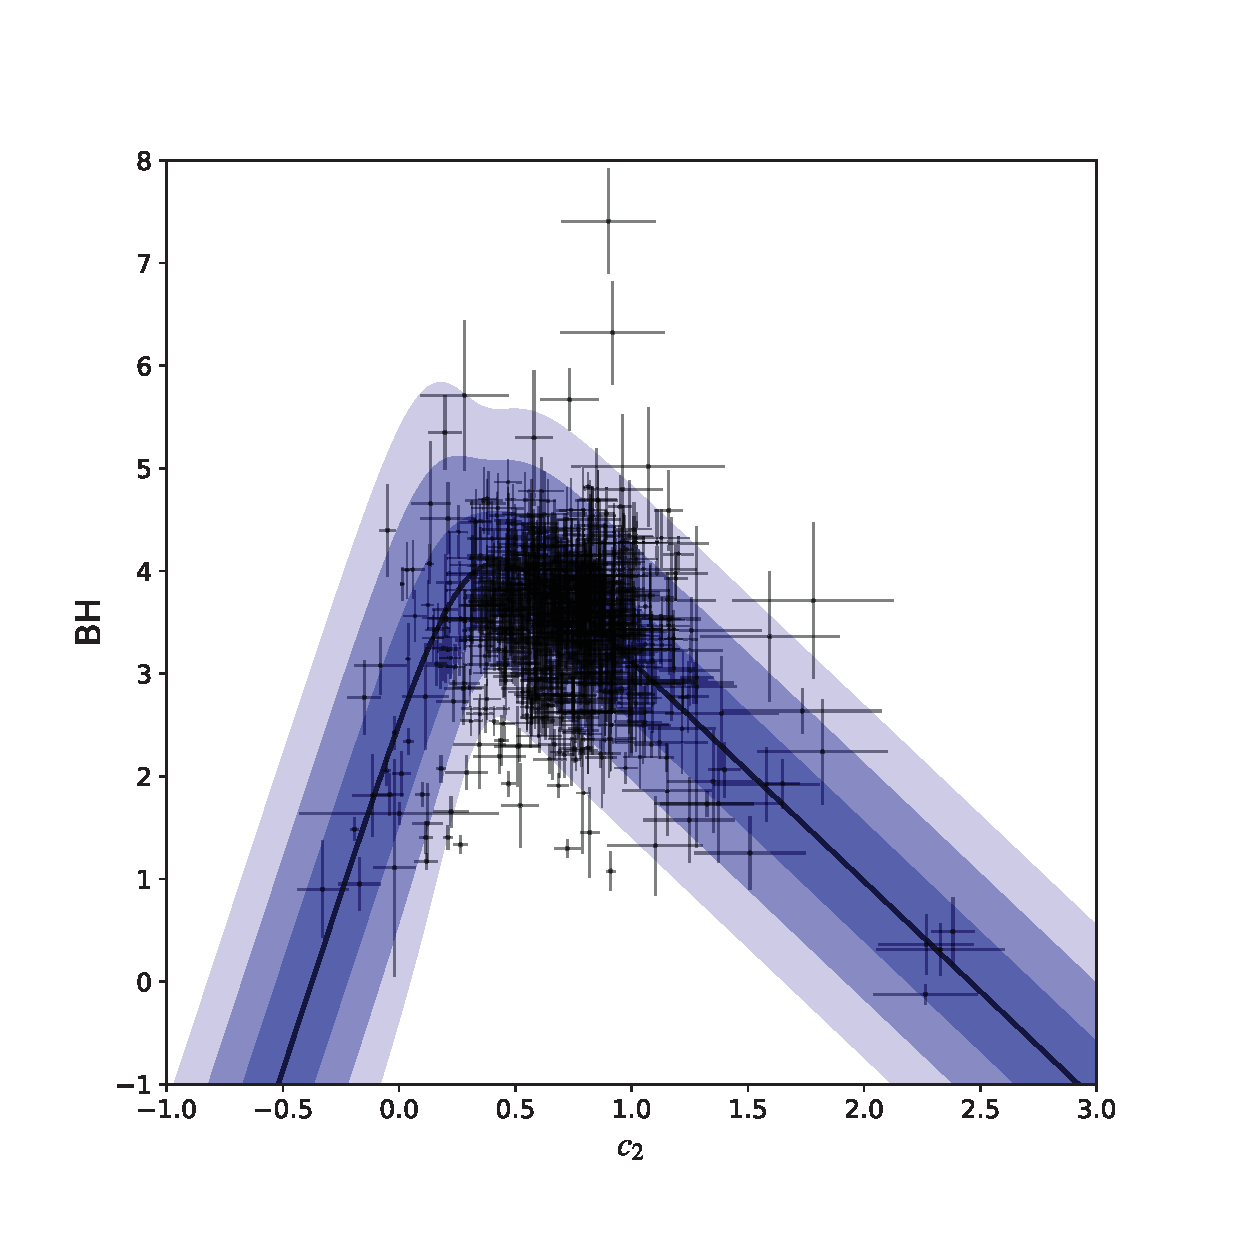
\includegraphics[width=1.0\linewidth]{figures/bhc2_data.eps}
    \caption{Observed $\text{BH}$ vs $c_2$ data from \textcite{valencic04}, \textcite{gordon03}, \textcite{newdatafitzpatrick2007analysis}, and \textcite{m31dataclayton2015new}, plotted with broken-linear TRK fit modeled by Equation \eqref{eq:bhc2model}. Shaded regions indicate the $1-$, $2-$ and $3\sigma$ slop confidence regions of the model distribution, given best fit slop values of Table \ref{table:bhc2} and plotted according to footnote \ref{footnote:modelcurvebands} on page \pageref{footnote:modelcurvebands}.}
    \label{fig:bhc2_data}
\end{figure}

\begin{figure}
    \centering
    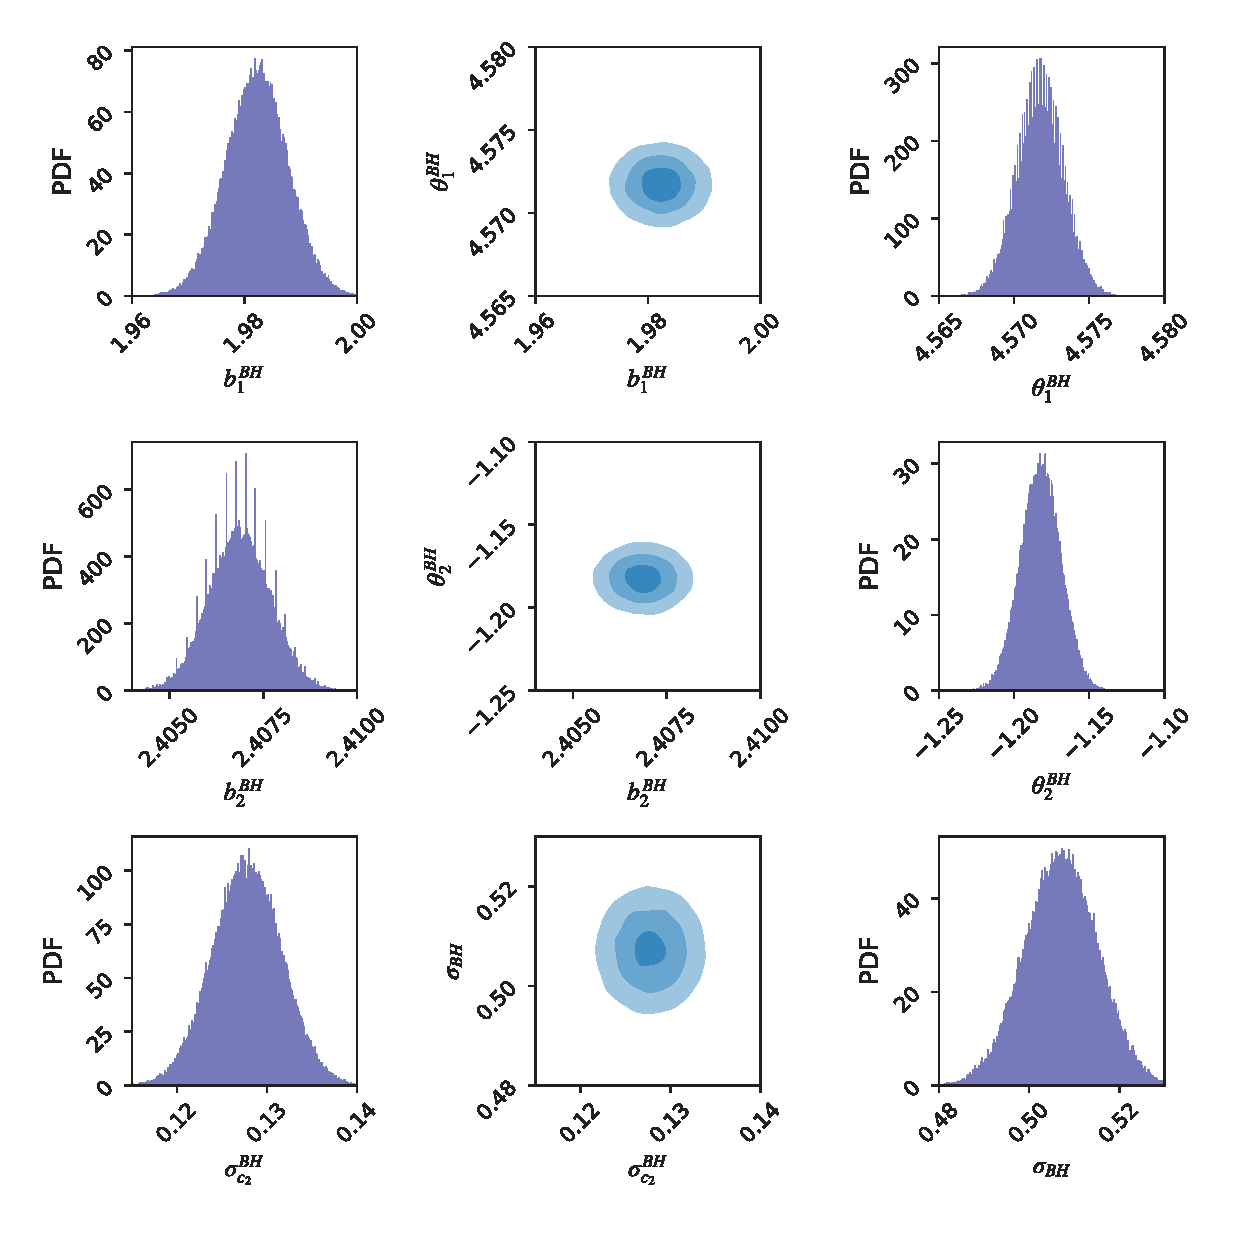
\includegraphics[width=1.0\linewidth]{figures/bhc2_params.eps}
    \caption{MCMC-generated (\S\ref{sec:MCMC}) probability distributions for $\text{BH}$ vs. $c_2$ (Equation \eqref{eq:bhc2model}) model (top and middle rows) and slop/extrinsic scatter (bottom row) parameters. Parameter confidence ellipses (center) with $1-$, $2-$ and $3\sigma$ regions show joint posterior probabilities with respect to the parameters plotted on either side. The pivot-point finding algorithm of \S\ref{sec:pivot} was used to remove respective correlations between model parameters of each linear "leg" of the model curve.}
    \label{fig:bhc2_params}
\end{figure}

\begin{table}
\label{table:bhc2}
\caption{Best-Fit Asymmetric Gaussian Parameter Values For $\text{BH}$ vs. $c_2$ Model (Equation \eqref{eq:bhc2model})}
\centering
\vspace{0.3cm}
\begin{tabular}{@{}lcccc@{}}
\toprule
Parameter Type   & Parameter            & Value    & \begin{tabular}[c]{@{}c@{}}$+1\sigma$\\ Width\end{tabular} & \begin{tabular}[c]{@{}c@{}}$-1\sigma$\\ Width\end{tabular} \\ \midrule
Model Parameters & $b_1^{\text{BH}}$            & 1.9837  &  0.0054                                                   &       $-0.0057$                      \\
                 & $\theta_1^{\text{BH}}$            & 4.5679  &  0.0016                                                    &    $-0.0015$                           \\
                 & $b_2^{\text{BH}}$            & 2.4040  &     0.0008                                                 &    $-0.0008$                                \\
                 & $\theta_2^{\text{BH}}$            & $-1.1344$  &  0.0130                                                    &   $-0.0138$                              \\
Pivot Points     & $c_2^{p_1,\text{BH}}$      & $-0.0867$ & $\ldots$                                                   & $\ldots$                                                   \\
                 & $c_2^{p_2,\text{BH}}$      & 1.3343 & $\ldots$                                                   & $\ldots$                                                   \\
Slop Parameters  & $\sigma_{c_2}^{\text{BH}}$ & 0.1290  &  0.0037                                                   &  $-0.0039$                                                  \\
                 & $\sigma_{\text{BH}}$       & 0.4954  &  0.0077                                                   & $-0.0081$                                                    \\
Optimum Scale    & $s_0$                & 0.28117  & $\ldots$                                                   & $\ldots$                                                   \\
Minimum Scale    & $a$                  & 0.11816  & $\ldots$                                                   & $\ldots$                                                   \\
Maximum Scale    & $b$                  & 0.94043  & $\ldots$                                                   & $\ldots$                                                   \\ \bottomrule
\end{tabular}
\end{table}

% \subsection{Fitting $R_V$ vs. $c_2$}
% \textcite{trotter} reported that the parameters $R_V$ and $c_2$ are loosely correlated, with low values of $c_2$ corresponding to very high values of $R_V$, and moderate or higher values of $c_2$ corresponding to the well known, approximately fixed value of $R_V\sim 3.1$. Trotter parameterized this relationship with a ``smoothly-broken linear'' model curve of the form 
% \begin{equation}\label{eq:rvc2model}
%     R_{V,c}(c_2;\vartheta_m)=\ln\left[\exp{{b_1^{R_V}+\tan\theta_1^{R_V}\left(c_2-c_2^{p_1,R_V}\right)}}+\exp{{b_2^{R_V}+\tan\theta_2^{R_V}\left(c_2-c_2^{p_2,R_V}\right)}}\right],
% \end{equation}
% where $\vartheta_m=\{b_1^{R_V}, \theta_1^{R_V}, b_2^{R_V}, \theta_2^{R_V}\}$ are the model parameters and $\{c_2^{p_1,R_V}, c_2^{p_2,R_V}\}$ are the pivot points of the model that determine the amount of correlation between $b_1^{R_V}$ and $\theta_1^{R_V}$, and $b_2^{R_V}$ and $\theta_2^{R_V}$, respectively.

% To fit this model to the dataset, I first ran the scale optimization algorithm of \S\ref{sec:scaleop} to determine the optimum fitting scale $s_0$. Next, I ran the parameter correlation removal/pivot point-finding algorithm of \S\ref{sec:pivot} to determine the pivot points $c_2^{p_1,R_V}$ and $c_2^{p_2,R_V}$ that minimizes the correlation between $b_1^{R_V}$ and $\theta_1^{R_V}$, and $b_2^{R_V}$ and $\theta_2^{R_V}$, respectively\footnote{Note that the pivot point-finding algorithm of \S\ref{sec:pivot} and Algorithm \ref{algo:pivotpoint} was only explicitly defined for models with a single pivot point. As such, I modified the code to allow for models that have multiple pivot points using a fairly straightforward generalization of Algorithm \ref{algo:pivotpoint}. Specifically, I used the MCMC-sampled pairs of slope and intercept parameters (line 6 of Algorithm \ref{algo:pivotpoint}) to compute and weight samples from successive distributions of possible pivot points (lines 8 through 17), in order to iteratively determine optimal values for the two pivot points (lines 19 and 20).}. From here, I determined the best fit model and $(x-,y-)$slop parameters $\vartheta_m=\{b^{c_1}, m^{c_1}\}$ and $(\sigma_{c_2}^{c_1}, \sigma_{c_1})$, respectively using the Downhill Simplex method of \S\ref{sec:simplex} at $s_0$\footnote{Note that I was able to run the scale optimization before finding the pivot point because fitting scales are invariant of choice of pivot point, as they don't affect the extreme scale limiting behavior of slops, e.g. \textcite{trotter}.}. Finally, I used the Adaptive MCMC and Bar-Lowering methods of \S\ref{sec:MCMC} to sample the distribution of the model and slop parameters, and compute their uncertainties, respectively. 

% The numerical results of this fit are given in Table \ref{table:c1c2}, while the fit is plotted in Figure \ref{fig:c1c2_data} with generated model and slop parameter distributions shown in Figure \ref{fig:c1c2_params}. In Figure \ref{fig:c1c2_data}, note the small slop confidence regions of the model distributiona about the model line, indicated a strong correlation between $c_1$ and $c_2$, as expected. Also, note that because the pivot point-finding routine was used to minimize the correlation between $b^{c_1}$ and $m^{c_1}$, the confidence ellipse for these two parameters (top, center of Figure \ref{fig:c1c2_params}) is not tilted, indicating the removal of correlation between them. Finally, also note in this figure that the two slop parameters $(\sigma_{c_2}^{c_1}$ and $\sigma_{c_1})$ are also uncorrelated, again evidenced by a non-tilted confidence ellipse (bottom, center).

% \begin{figure}
%     \centering
%     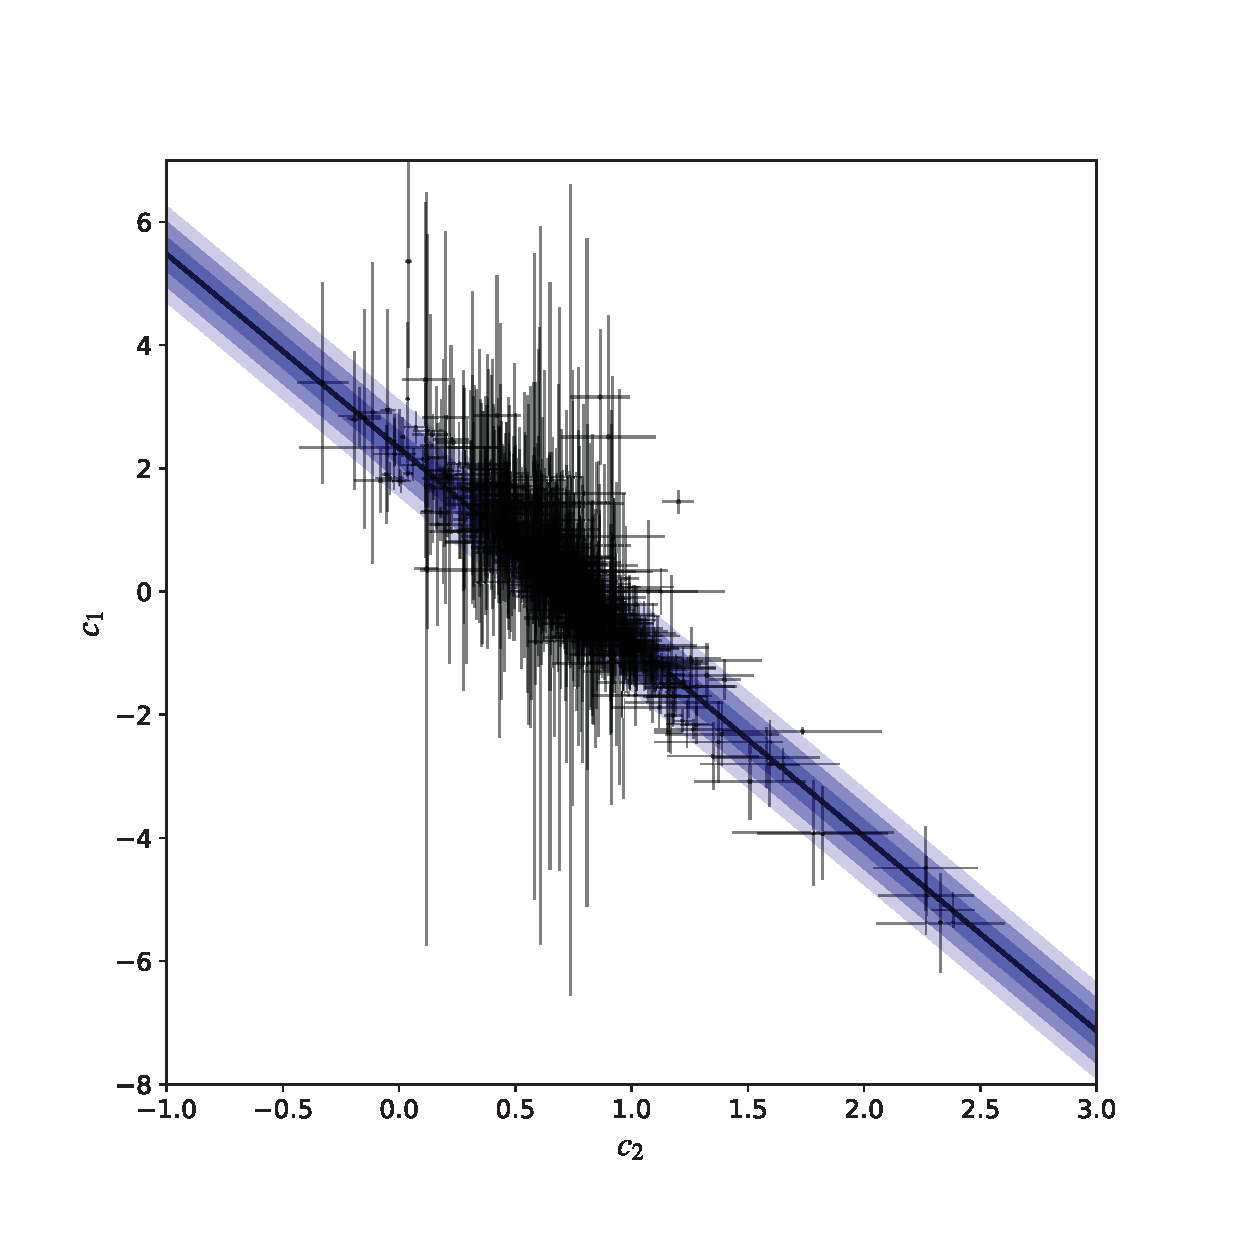
\includegraphics[width=1.0\linewidth]{figures/c1c2_data.eps}
%     \caption{Observed $R_V$ vs $c_2$ data from \textcite{valencic04}, \textcite{gordon03}, \textcite{newdatafitzpatrick2007analysis}, and \textcite{m31dataclayton2015new}, plotted with broken-linear TRK fit modeled by Equation \eqref{eq:rvc2model}. Shaded regions indicate the $1-$, $2-$ and $3\sigma$ slop confidence regions of the model distribution, given best fit slop values of Table \ref{table:rvc2} and plotted according to \ref{footnote:modelcurvebands} on page \pageref{footnote:modelcurvebands}.}
%     \label{fig:rvc2_data}
% \end{figure}

% \begin{figure}
%     \centering
%     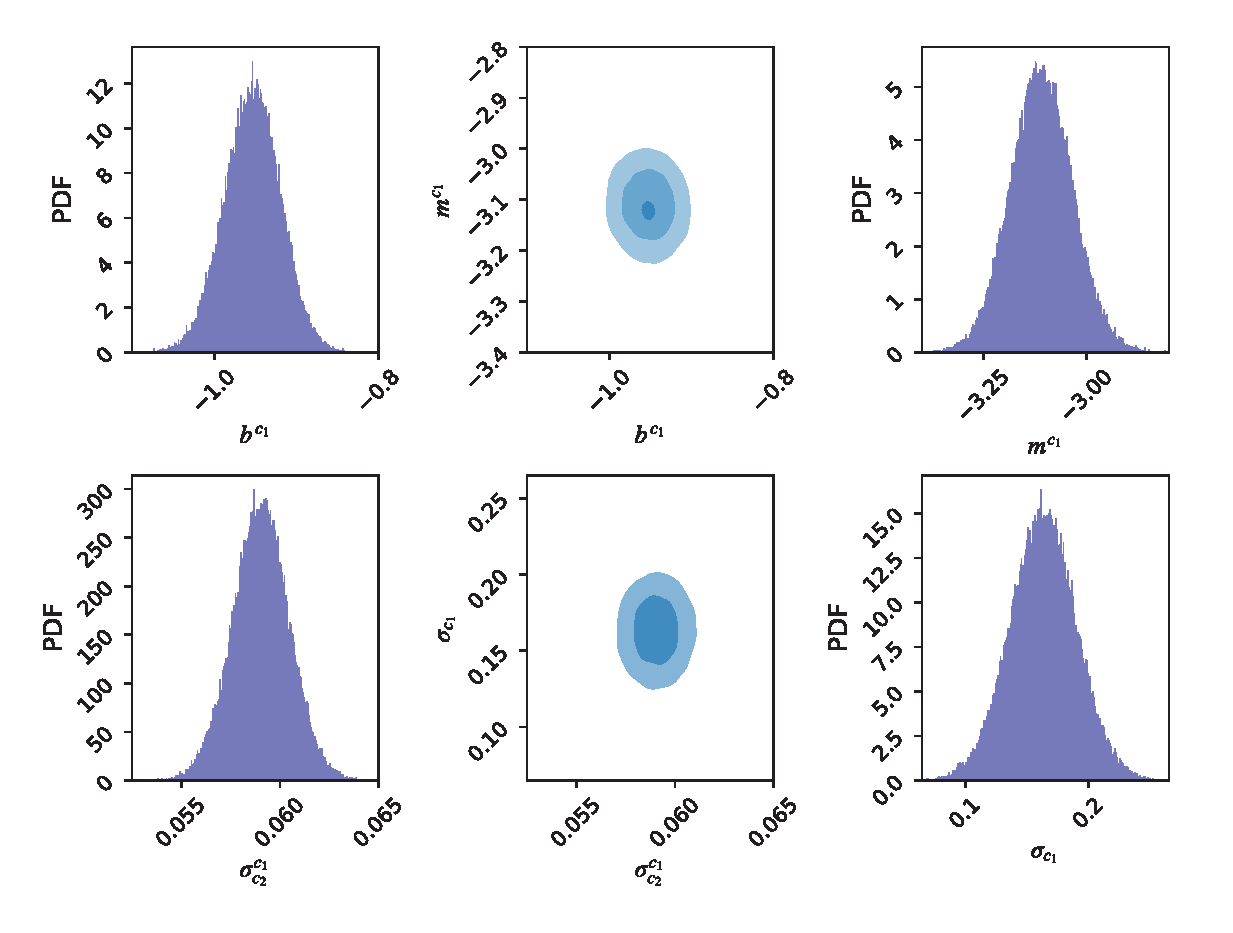
\includegraphics[width=1.0\linewidth]{figures/c1c2_params.eps}
%     \caption{MCMC-generated (\S\ref{sec:MCMC}) probability distributions for $R_V$ vs. $c_2$ (Equation \eqref{eq:rvc2model}) model (top and middle rows) and slop/extrinsic scatter (bottom row) parameters. Parameter confidence ellipses (center) with $1-$, $2-$ and $3\sigma$ regions show joint posterior probabilities with respect to the parameters plotted on either side. The pivot-point finding algorithm of \S\ref{sec:pivot} was used to remove respective correlations between model parameters of each linear "leg" of the model curve.}
%     \label{fig:rvc2_params}
% \end{figure}

% \begin{table}
% \label{table:c1c2}
% \caption{Best-Fit Asymmetric Gaussian Parameter Values For $R_V$ vs. $c_2$ Model (Equation \eqref{eq:rvc2model})}
% \centering
% \vspace{0.3cm}
% \begin{tabular}{@{}lcccc@{}}
% \toprule
% Parameter Type   & Parameter            & Value    & \begin{tabular}[c]{@{}c@{}}$+1\sigma$\\ Width\end{tabular} & \begin{tabular}[c]{@{}c@{}}$-1\sigma$\\ Width\end{tabular} \\ \midrule
% Model Parameters & $b_1^{R_V}$            &   &                                                     &                             \\
%                  & $\theta_1^{R_V}$            &   &                                                      &                               \\
%                  & $b_2^{R_V}$            &   &                                                      &                                    \\
%                  & $\theta_2^{R_V}$            &   &                                                      &                                 \\
% Pivot Points     & $c_2^{p_1,R_V}$      &  & $\ldots$                                                   & $\ldots$                                                   \\
%                  & $c_2^{p_2,R_V}$      &  & $\ldots$                                                   & $\ldots$                                                   \\
% Slop Parameters  & $\sigma_{c_2}^{R_V}$ &   &                                                     &                                                    \\
%                  & $\sigma_{R_V}$       &    &                                                      &                                                     \\
% Optimum Scale    & $s_0$                &   & $\ldots$                                                   & $\ldots$                                                   \\
% Minimum Scale    & $a$                  &   & $\ldots$                                                   & $\ldots$                                                   \\
% Maximum Scale    & $b$                  &   & $\ldots$                                                   & $\ldots$                                                   \\ \bottomrule
% \end{tabular}
% \end{table}

\section{A Web-Based TRK Fit Calculator}
\label{sec:website}
Alongside with the development of the TRK suite source code, the other main project that I undertook is the end-to-end development of a web-based calculator for running TRK fits, currently located at \url{https://skynet.unc.edu/rcr/calculator/trk}\footnote{Note that this is part of the website that also includes the two Robust Chauvenet Outlier Rejection (RCR) calculators (see \textcite{maples2018robust}), that I am also the developer of (both the RCR source code and webpages). Long term, I plan to develop a single standalone statistical suite, available in multiple languages, that will bring together RCR, TRK, and other future statistical tools that I've developed, of which this website will be part of the ecosystem of.}. Easy to use, but full of customization options, the goal of this website was to create a simple, user-friendly introduction to the TRK statistic, including educational interactive visualization tools.

The first step of the web-based TRK calculator is to input the raw data, shown in Figure \ref{fig:websiteinput}, where the user can give values for $\{x_n,\sigma_{x,n},y_n,\sigma_{y,n}\}$ with optional weights $\{w_n\}$.
\begin{figure}
    \centering
    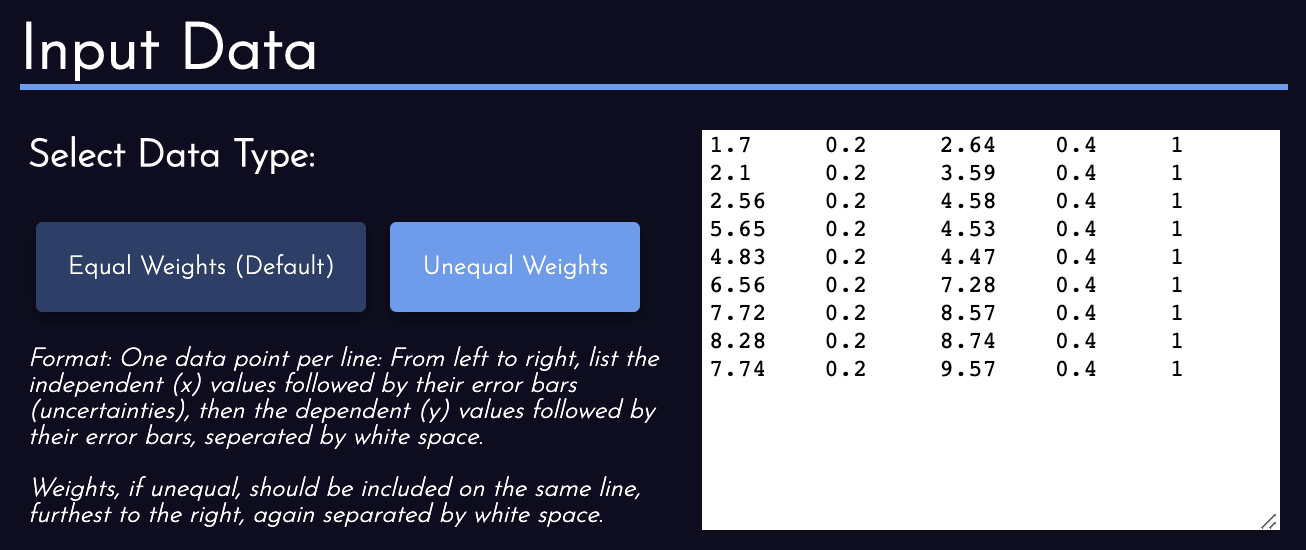
\includegraphics[width=1.0\linewidth]{figures/websiteinput.png}
    \caption{The data input step of the web-based TRK calculator with example data.}
    \label{fig:websiteinput}
\end{figure}
Next, shown in Figure \ref{fig:websiteinputplot}, the user can plot the data with error bars in order to estimate which model to fit to the data. The plot also offers various interactive tools, including the ability to pan and zoom\footnote{This plot, as well as all other plots on the TRK and RCR webpages, were made with Python's Bokeh library, from the \textcite{bokeh}.}.
\begin{figure}
    \centering
    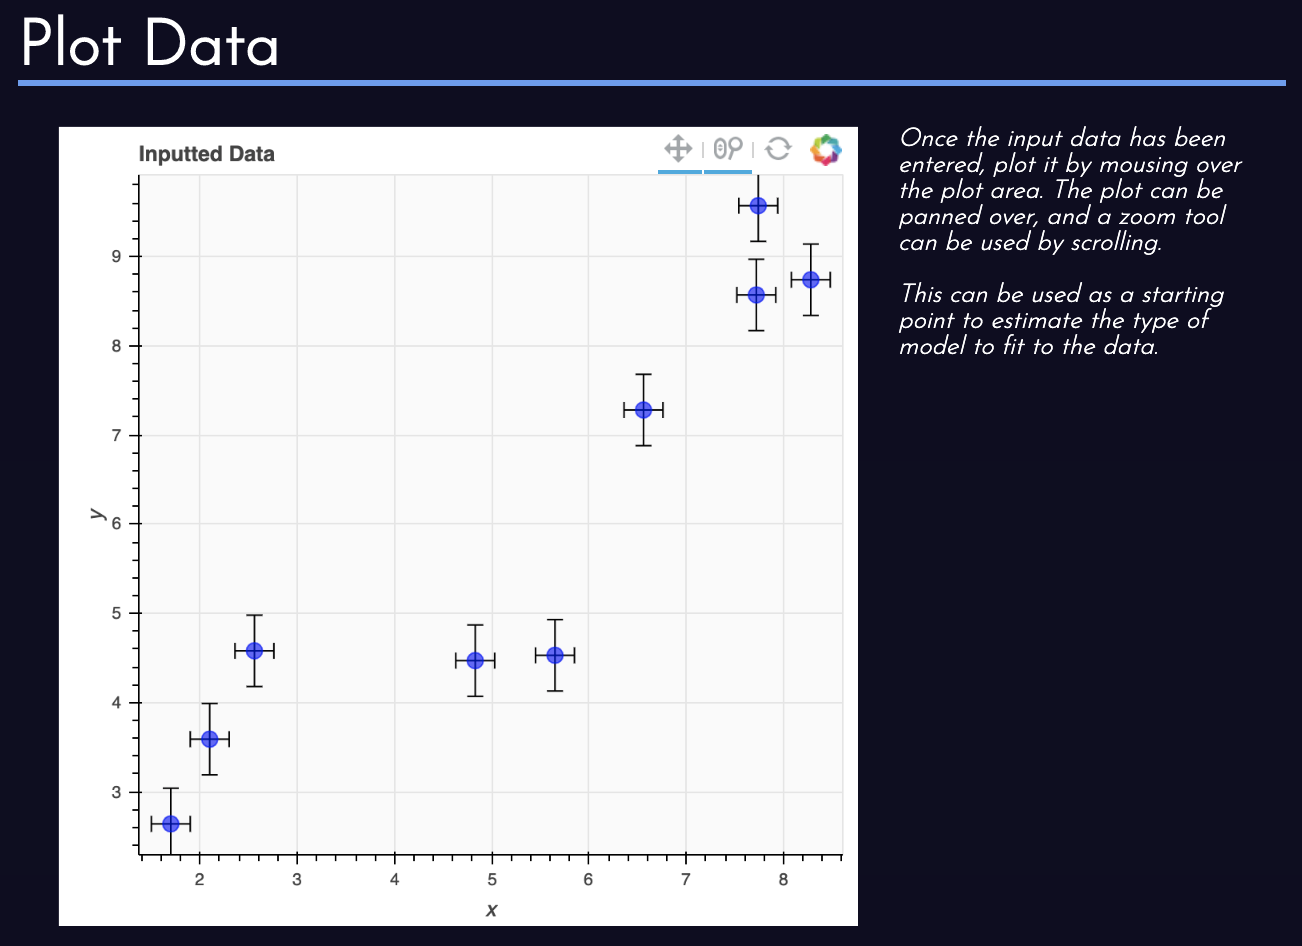
\includegraphics[width=1.0\linewidth]{figures/websiteinputplot.png}
    \caption{Example of plotting input data on the TRK calculator webpage.}
    \label{fig:websiteinputplot}
\end{figure}

The following step is then for the user to choose the model to fit the data to, shown in Figure \ref{fig:websitechoosemodel}, and to provide an initial guess for the model and slop parameters for the fitting algorithm. The website comes with six built-in models: linear, quadratic, cubic, exponential, power law and logarithmic; the user also has the option to run the pivot-point finding/de-correlation algorithm of \S\ref{sec:pivot} on applicable models.
\begin{figure}
    \centering
    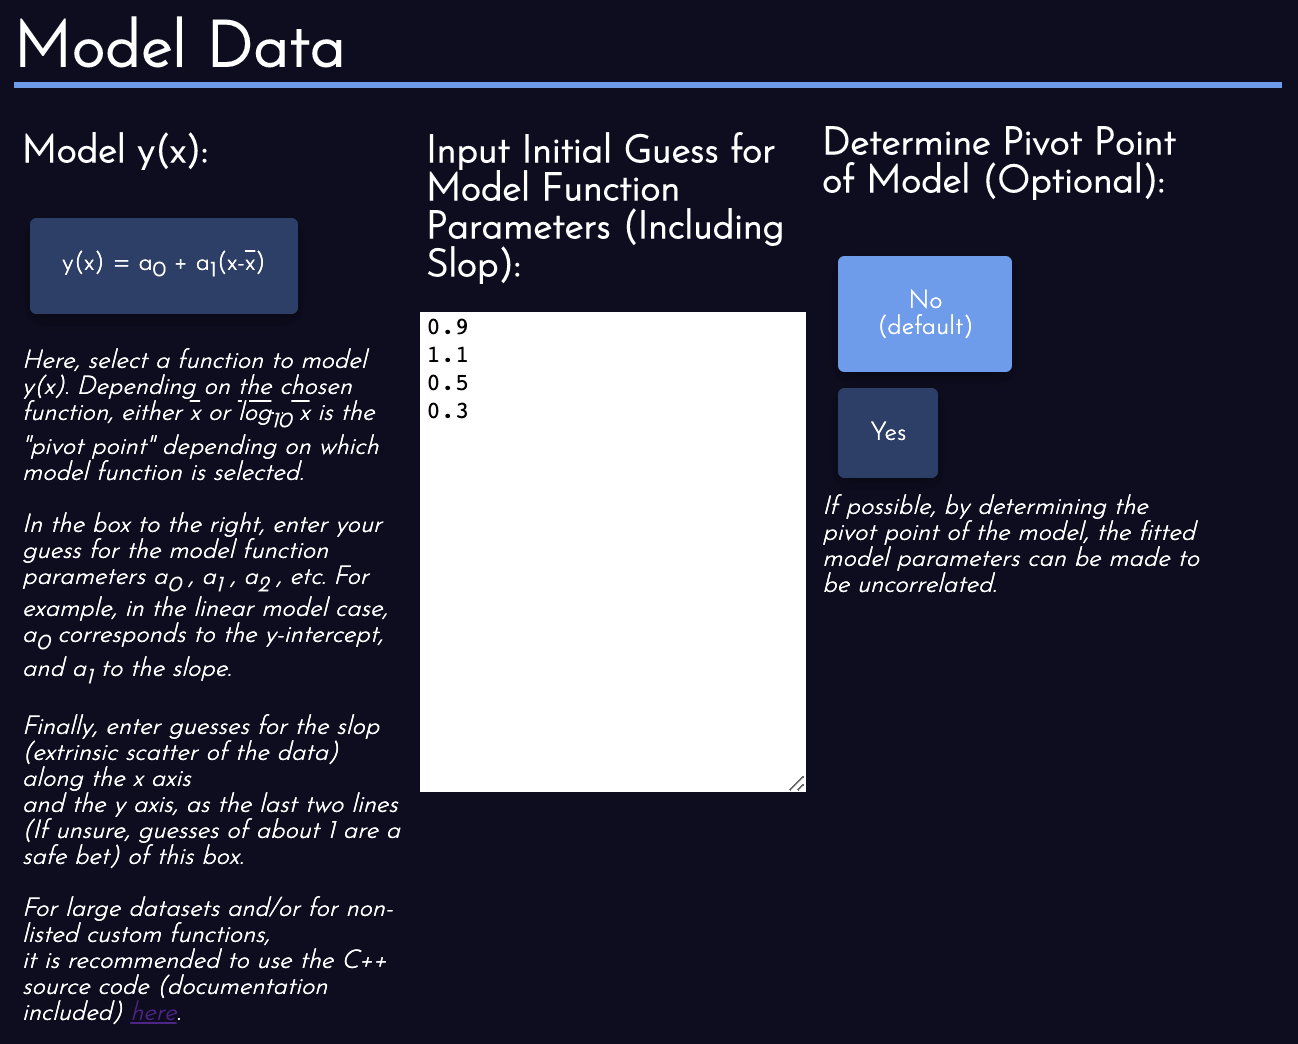
\includegraphics[width=1.0\linewidth]{figures/websitechoosemodel.png}
    \caption{Section of the TRK webpage where the user can choose which model to fit to their data.}
    \label{fig:websitechoosemodel}
\end{figure}

The last step of the calculator is for the user to choose which algorithms, if any, to run in addition to the regular likelihood-maximization downhill-simplex fitting of \S\ref{sec:simplex}, shown in Fig. \ref{fig:websitechoosealgo}. The user can choose to either provide a fitting scale $s$ (with a default of $s=1.0$), or run the scale optimization algorithm. The user also has the option to use the MCMC algorithm of \S\ref{sec:MCMC} to determine model parameter uncertainties; however, this is a computationally intensive process, so I am still experimenting with the possibility of expediting it. As shown, the total selected algorithm is displayed as a flow chart, with bullet-points below explaining the various steps\footnote{As shown, these bullet points also show section numbers; these correspond to the relavent sections of our upcoming paper, \textcite{TRKIapjs}, that will introduce the TRK statistic and some of its astrophysical applications in a peer-reviewed, journalistic context. The paper, currently in preparation, will be submitted to the Astrophysical Journal, Supplement Series.}.
\begin{figure}
    \centering
    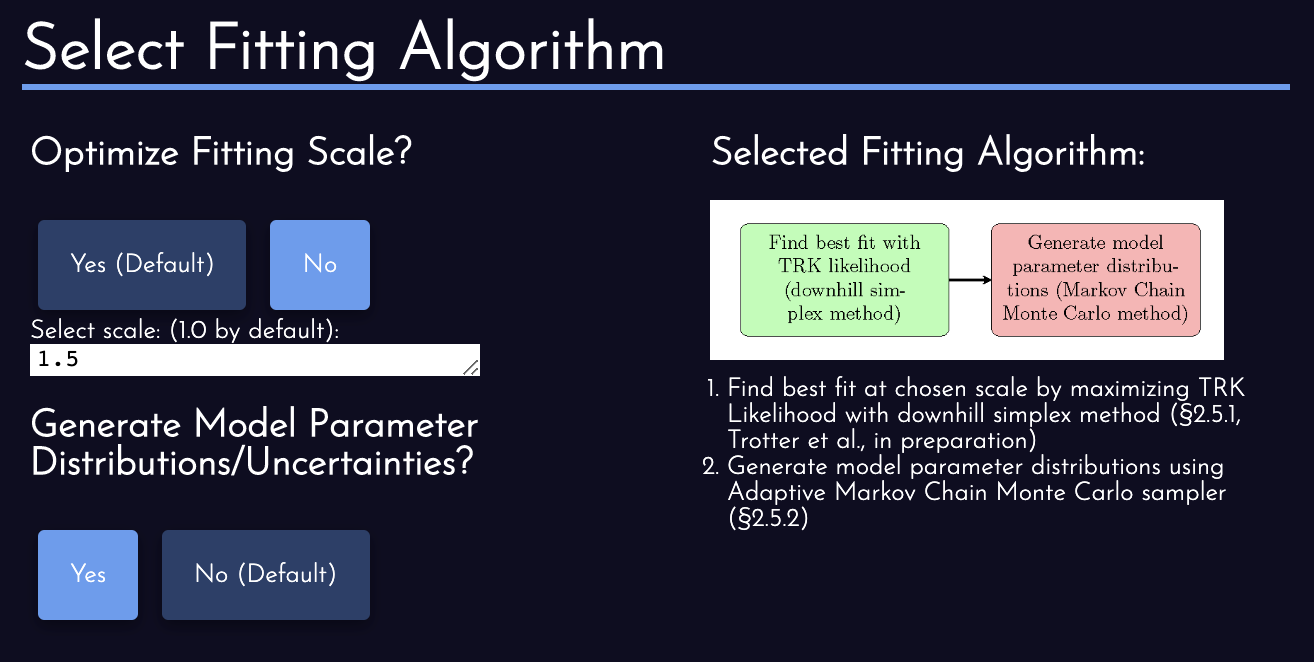
\includegraphics[width=1.0\linewidth]{figures/websitechoosealgo.png}
    \caption{Section of the TRK webpage where the user can determine which additional TRK algorithms to run alongside basic fit.}
    \label{fig:websitechoosealgo}
\end{figure}

With these steps completed, the user can now perform a TRK Fit, in the section shown in Figure \ref{fig:websiteoutput}. After pressing the ``Perform Fit'' button and waiting for the algorithm to run, the final model and slop parameters are displayed on the left, as shown (with the model parameters ordered according to the functional form of the chosen model). If the scale optimization algorithm was run, the optimum and extreme scales, $(s_0,a,b)$, respectively, will also be displayed. The resulting fitted model curve is then plotted alongside the data, including 1-, 2- and $3\sigma$ confidence regions described by the fitted slop parameters (see Footnote \ref{footnote:modelcurvebands} on page \pageref{footnote:modelcurvebands} to see how these regions are explicitly calculated).
\begin{figure}
    \centering
    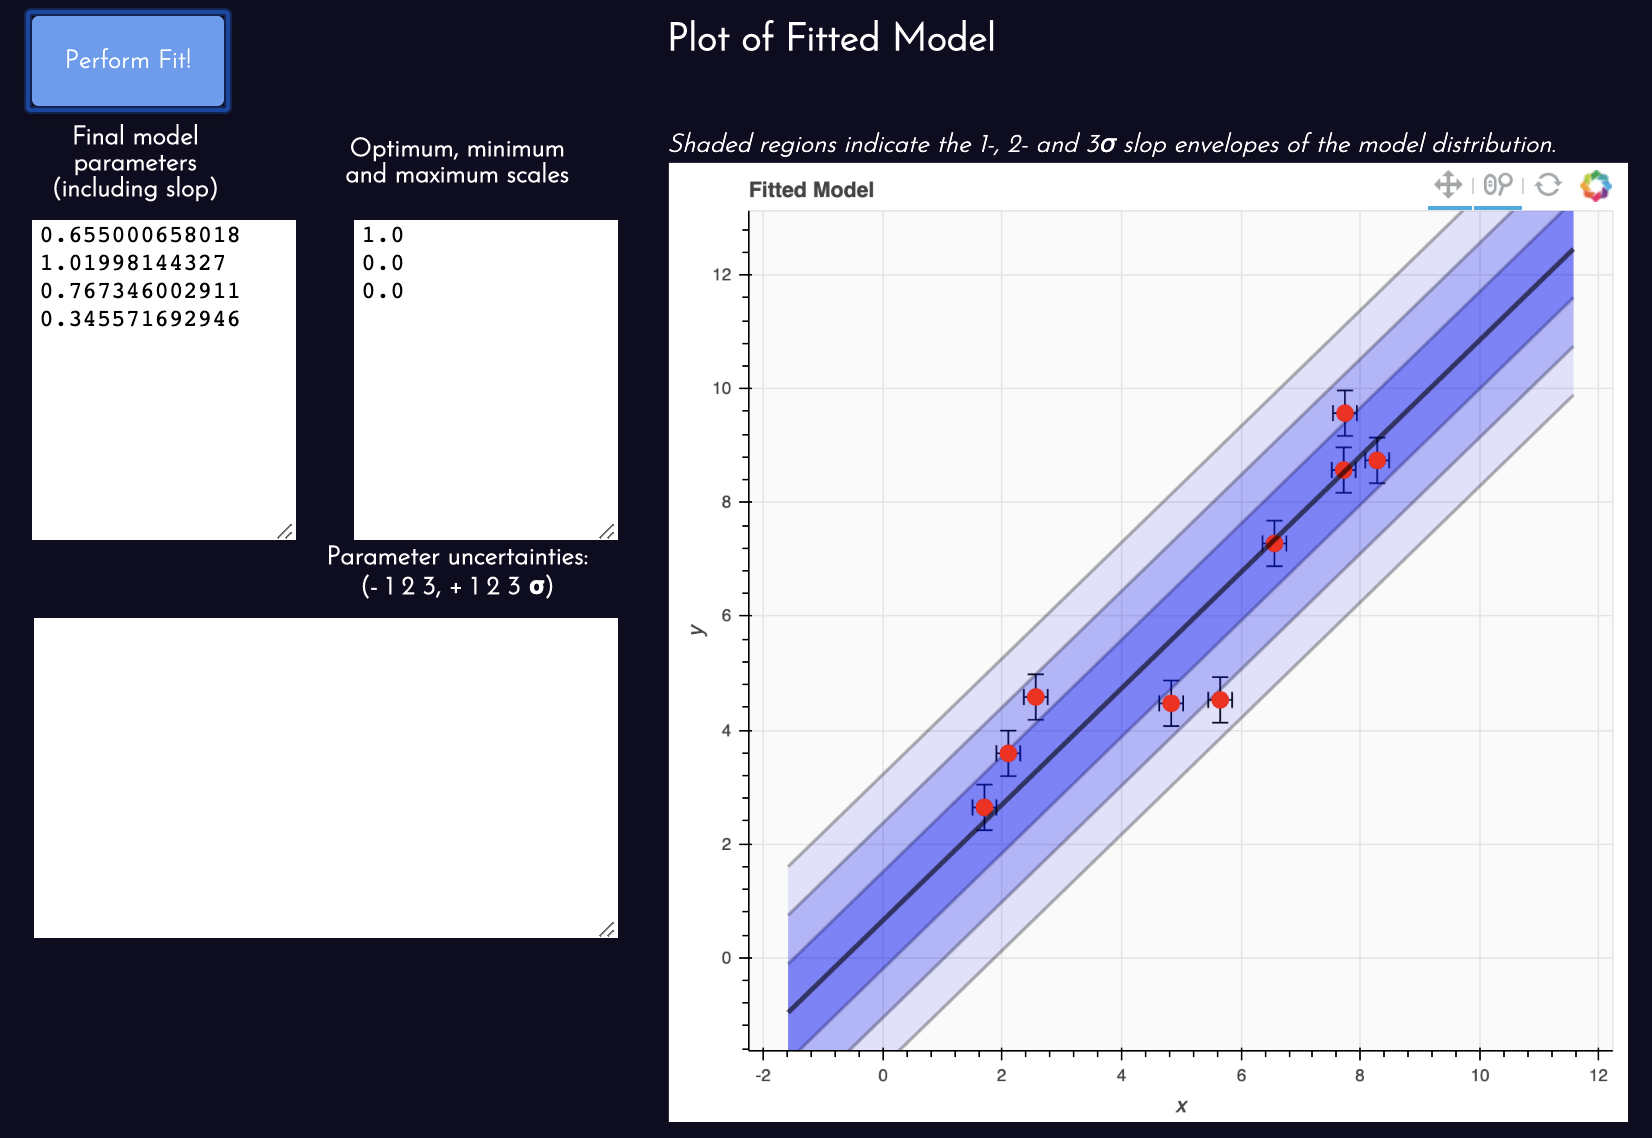
\includegraphics[width=1.0\linewidth]{figures/websiteoutput.png}
    \caption{Output section of the TRK calculator webpage, showing the results of an example linear fit (without model parameter uncertainty computation).}
    \label{fig:websiteoutput}
\end{figure}